\label{chap:programming_language_concepts}

\begin{abstract}
    Poglavlje ćemo započeti sa konceptom klasa\index{klasa} i objekata\index{objekt} kao temeljnim blokovima objektno-orijentirane paradigme\index{Objektno-orijentirana paradigma} programiranja. Zapravo je naglasak cijelog poglavlja na klasama i objektima. Bez poznavanja tog koncepta kao i cijele objektno-orijentirane paradigme je nemoguće programirati u Java programskom jeziku.
    
    Nakon što smo objasnili klase i objekte objasniti ćemo i aplikacijsko programsko sučelje. U sekciji \ref{sec:java_platform} spominjali smo Java API no ovdje ćemo isti definirati i objasniti.
\end{abstract}

\section{Koncept klasa i objekata}
Teorija objektno orijentiranog programiranja je bila obrađena u dijelu "Uvod u programiranje" tako da ćemo ovdje opisivati način na koji je objektno orijentirano programiranje implementirano u sam Java programski jezik.

Java programski jezik je "pravi" objektno orijentirani programski jezik. Zašto "pravi"? Zato što je koncept objektno orijentiranog programiranja objedinjen u programski jezik Java, tj. sve u Javi je objekt. Primjerice, Python, PHP i C++ programski jezici u sebi imaju ugrađenu objektno orijentiranu paradigmu no oni vam ipak dozvoljavaju da istu i ne koristite. Dakle programer, u takvih programskim jezicima, za svoje potrebe može koristiti isključivo proceduralnu paradigmu programiranja.

Drugim riječima, da bi počeli objašnjavati programski jezik Java moramo ipak malo i proći kroz koncept objektno orijentiranog programiranja.

\subsection{Objekti}
Objekti\index{objekt} su srce objektno orijentirane paradigme programiranja. Objekt\index{objekt} je softverska komponenta koji ima svoje stanje\index{objekt!stanje} i ponašanje\index{objekt!ponašanje}, tj. funkcionalnost. Ako pogledamo ovaj naš stvarni svijet, vidjet ćemo mnogo primjera objekata; stolna svjetiljka, automobil, televizor, mikrovalna pećnica, itd.. I ako malo razmislimo, svaki taj objekt iz stvarnog svijeta ima svoje stanje i ponašanje.

Televizor, primjerice, može biti uključen ili isključen. Može biti podešen da trenutno prikazuje signal s antene i da prikazuje HRT 2. Mikrovala pećnica, kada se podesi da zagrijava hranu, odbrojava do trenutka kada treba prestati zagrijavati. Dakle, to su sve nekakva stanja u kojima ti objekti mogu biti. Televizor i mikrovalna pećnica isto tako mogu imati i svoje ponašanje. Primjerice, televizor možete uključiti i isključiti, pojačati i stišati glasnoću. Mikrovalnoj pećnici možete "narediti" da odledi zaleđenu hranu ili da ispeče cijelo pile. Ono što je bitno za primijetiti je da ponašanje objekta zapravo mijenja njegovo stanje. Drugim riječima, nije isto ako hoćete da pećnica odleđuje hranu ili da ispeče pile; ovisno o odabiru parametri se mijenjaju. Pećnica će se, prema vašem odabiru, "sama podesiti". Odredit će snagu i vrijeme koje treba da obavi posao koji ste htjeli. Dakle još jednom - ovisno o odabranom ponašanju ili funkciji objekt će mijenjati svoja stanja.

\begin{infobox}
    Objekti imaju svoje stanje\index{objekt!stanje} i ponašanje\index{objekt!ponašanje} tj., funkcije.
\end{infobox}

U programskom jeziku Java objekti svoje stanje\index{objekt!stanje} spremaju u varijable (eng. \emph{fields}\index{objekt!\emph{fields}}), a svoje ponašanje\index{objekt!ponašanje} definiraju pomoću funkcija ili metoda (eng. \emph{methods}\index{objekt!\emph{methods}}). Objektom upravljamo pomoću definiranih metoda te na takav način objektu mijenjamo njegovo stanje.

Slika~\ref{fig:object_conceptual_model} ispod prikazuju konceptualni model objekta.~\cite{javatutorials}

\begin{figure}[!htbp]
    \caption{Konceptualni model objekta.}
    \label{fig:object_conceptual_model}
    \centering
    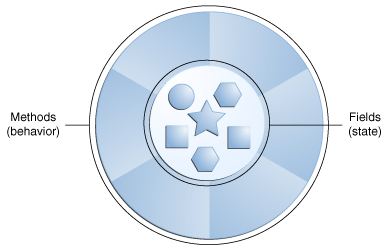
\includegraphics[scale=0.6]{images/object_conceptual_model.png}
\end{figure}

Vratimo se na primjer mikrovalne pećnice. Ako softverskim objektom komuniciramo pomoću njegovih metoda onda komunikaciju s mikrovalnom pećnicom obavljamo preko njezinih kontrola smještenih na kontrolnoj ploči koja se nalazi odmah pored vratašca. Ako malo bolje primijetimo, zapravo, ne postoji nijedan drugi način komunikacije s pećnicom osim sa spomenutom kontrolnom pločom. Inženjeri, koji su osmislili tu mikrovalnu pećnicu, su vama dali samo nekoliko funkcija na korištenje. Dakle, vi kao korisnik pećnice jedino trebate znati ponuđene funkcije. Sve ostalo je od vas sakriveno u samom kućištu mikrovalne pećnice. Niti znate što je sve u tom kućištu niti vas i zanima. Vas jedino zanima tih par dugmeta na kontrolnoj ploči.

Drugim riječima, inženjeri su sakrili kompleksnost same mikrovalne pećnice te vama tako olakšali posao. Ista analogija vrijedi i za softverske objekte. Dakle, programer objekta je ponudio vama na korištenje samo neki određeni set metoda. I jedino pomoću tih metoda vi zapravo možete upravljati tim objektom. Vas nezanima šta te metode onda konkretno rade. Bitno je da vi znate šta ćete postići korištenjem tih metoda.

Drugim riječima, stanje objekta je zaštićeno pomoću tih metoda i na takav način objekt, zapravo, kontrolira kako će ga vanjski svijet koristiti. To načelu u objektno orijentiranoj paradigmi se naziva enkapsulacija\index{enkapsulacija} (eng. \emph{encapsulation}\index{\emph{encapsulation}}).

Primjer enkapsulacije\index{enkapsulacija} je model~\cite{javatutorials} bicikla i njegova metoda \texttt{changeGears()}. Ako bicikl ima 18 brzina onda ta metoda može odbiti promijeniti brzinu ako je vrijednost koju pošaljemo objektu manja od 1 ili veća od 18. Inače bi taj objekt koji predstavlja bicikl zapravo doveli u inkonzistentno stanje.

\begin{figure}[!htbp]
    \caption{Konceptualni model bicikla.}
    \label{fig:bicycle_conceptual_model}
    \centering
    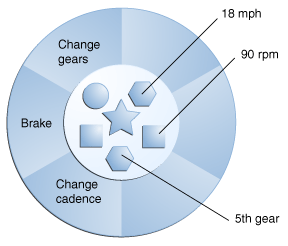
\includegraphics[scale=0.6]{images/bicycle_conceptual_model.png}
\end{figure}

U stvarnom svijetu, aplikacije su nerijetko kompleksne te imaju na tisuće i tisuće objekata. Slika~\ref{fig:oop_system_abstract_overview} prikazuje apstraktni prikaz aplikacije koja koristi objekto orijentiranu paradigmu\index{Objektno-orijentirana paradigma} u svojem razvoju. Iz slike se može vidjeti da se aplikacija sastoji od mnoštva objekata koji su povezani u logične cjeline te kao takvi komuniciraju jedno s drugim da bi obavili svoj zadatak za kojeg su i programirani.

\begin{figure}[!htbp]
    \caption{Apstraktni prikaz objekto-orijentirane paradigme\index{Objektno-orijentirana paradigma}.}
    \label{fig:oop_system_abstract_overview}
    \centering
    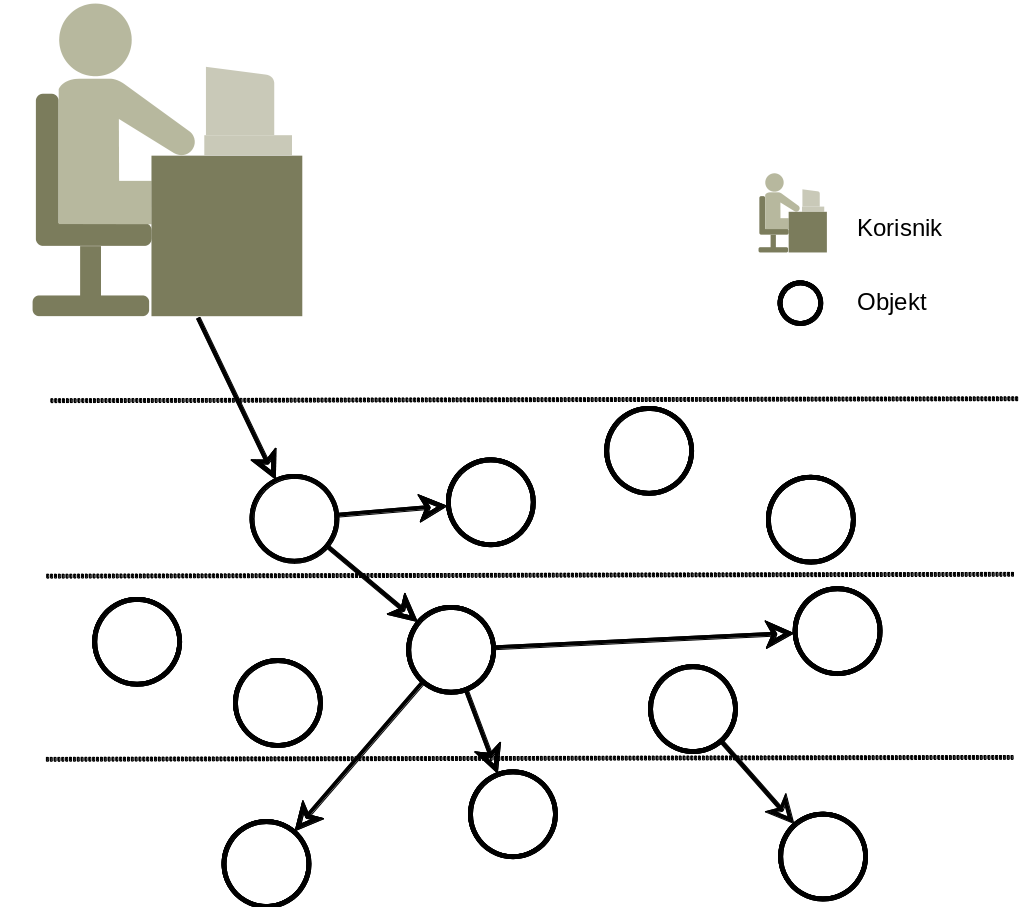
\includegraphics[scale=0.4]{images/oop_system_abstract_overview.png}
\end{figure}

Dakle, svaki taj objekt ima svoju ulogu u aplikaciji. Važno je da se cijela poslovna logika aplikacije koju razvijate podijeli u neke logične cjeline. Zatim da se za svaku logičnu cjelinu prepoznaju objekti koji će odraditi neki dio posla. U objekto orijentiranom programiranju\index{Objektno-orijentirana paradigma} je od najviše važnosti da se enkapsulacija svakog objekta drži na visokoj razini. Drugim riječima, najvažnije je da se sakriju detalji implementacije objekta te da se njegova stanja isključivo mogu mijenjati preko njegovih metoda.

\subsection{Klase}
Java je \emph{class-based}\index{\emph{class-based}} \cite{classbasedprogramming} programski jezik. U istu grupu spadaju i Python, PHP i C++ programski jezici. Dok primjerice JavaScript, Lua i Ruby, koji su također objektno orijentirani programski jezici, pripadaju u grupu \emph{prototype-based}\index{\emph{prototype-based}} \cite{prototypebasedprogramming} programskih jezika.

Poznavanje gore dvije spomenute terminologije nije bitno; bitno je znati da u programskom jeziku Java, \emph{class-based}\index{\emph{class-based}} stil programiranja znači da je svaki objekt određen s klasom. Drugim riječima - ne postoji način da dobijete objekt ako nemate njegovu klasu.

E sad, šta je to klasa? U stvarnom svijetu često ćete naići na objekte iste vrste; postoje na tisuće automobila koje su zapravo iste marke i modela. Svaki od tih automobila je napravljen od istog nacrta stoga su oni građeni od istih komponenti i imaju iste karakteristike i mogućnosti.

U objektno orijentiranoj terminologiji mi kažemo da je svaki taj automobil instanca (eng. \emph{instance}) iste klase (eng. \emph{class}). Dakle, klasa\index{klasa} je nacrt (eng. \emph{blueprint}) od koje se svaki objekt stvoren. Definicija klase određuje mogućnosti svakog objekta te klase.

Sljedeći kôd predstavlja klasu i ona je jedna od mogućih implementacija bicikla:~\cite{javatutorials}

\begin{lstlisting}[language=java, caption=Bicycle]
class Bicycle {
    int cadence = 0;
    int speed = 0;
    int gear = 1;
    
    void changeCadence(int newValue) {
        cadence = newValue;
    }
    
    void changeGear(int newValue) {
        gear = newValue;
    }
    
    void speedUp(int increment) {
        speed = speed + increment;
    }
    
    void applyBrakes(int decrement) {
        speed = speed - decrement;
    }
    
    void printStates() {
        System.out.println("cadence:" + cadence + " speed:" + speed + " gear:" + gear);
    }
}
\end{lstlisting}

Naravno da je, u ovom trenutku, kôd iznad totalno nepoznat. No promotrite dizajn te klase i prisjetite se što smo pričali u poglavlju prije. Svaki objekt ima svoja stanja\index{objekt!stanje} i metode\index{objekt!ponašanje}. U ovom slučaju, varijable \texttt{cadence}, \texttt{speed} i \texttt{gear} predstavljaju stanja objekta i \texttt{changeCadence()}, \texttt{changeGear()}, \texttt{speedUp()}, \texttt{applyBrakes()} i \texttt{printStates()} predstavljaju metode objekta.

Kao što je i rečeno, da bi se koristila ta klasa vi morate od nje napraviti objekt. Dakle, morate napraviti instancu te klase. Sljedeći kôd predstavlja također jednu klasu koja zapravo koristi klasu \texttt{Bicycle}.~\cite{javatutorials}

\begin{lstlisting}[language=java, caption=BicycleDriver]
class BicycleDriver {
    public static void main(String[] args) {
        // Create two different Bicycle objects
        Bicycle bike1 = new Bicycle();
        Bicycle bike2 = new Bicycle();
        
        // Invoke methods on those objects
        bike1.changeCadence(50);
        bike1.speedUp(10);
        bike1.changeGear(2);
        bike1.printStates();
        
        bike2.changeCadence(50);
        bike2.speedUp(10);
        bike2.changeGear(2);
        bike2.changeCadence(40);
        bike2.speedUp(10);
        bike2.changeGear(3);
        bike2.printStates();
    }
}
\end{lstlisting}

\section{Aplikacijsko programsko sučelje}